\documentclass{standalone}
\usepackage{fontspec}
\usepackage{tikz}
\usepackage{bm}
\renewcommand*\familydefault{\sfdefault}
%\usepackage{sansmath}%\usepackage{arev}
\usepackage[italic]{mathastext}
\usepackage{isomath}
%\setromanfont{CMU Sans Serif}

\begin{document}
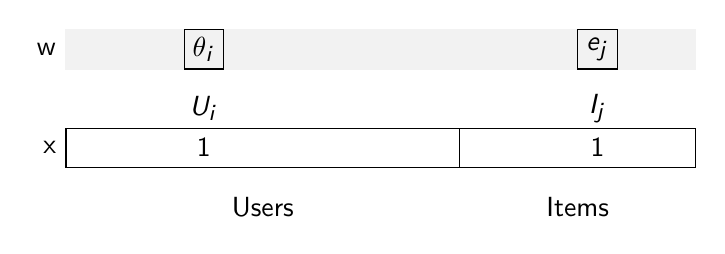
\begin{tikzpicture}[scale=0.5]
\filldraw[gray!10!white] (0,2.5) rectangle ++(16,1);
\draw (0,0) rectangle (16,1);
\draw node[left] at (0,0.5) {$\bm{x}$};
\draw node[left] at (0,3) {$\bm{w}$};
\node at (3.5,0.5) {1};
\node at (3.5,3) {$\theta_i$};
\node at (13.5,0.5) {1};
\node at (13.5,3) {$e_j$};
\node at (3.5,1.5) {$U_i$};
\node at (13.5,1.5) {$I_j$};

\draw (3,2.5) rectangle ++(1,1);
\draw (13,2.5) rectangle ++(1,1);
\draw (10,0) -- ++(0,1);
\node at (5,-1) {Users};
% \node at (5,4) {$\theta$};
\node at (13,-1) {Items};
% \node at (13,4) {$e$};
%\draw (3,4) rectangle ++(1,3);
\end{tikzpicture}
\end{document}
